\chapter{\ifenglish Introduction\else บทนำ\fi}

\section{\ifenglish Project rationale\else ที่มาของโครงงาน\fi}
การวัดความสูงของต้นไม้เป็นข้อมูลพื้นฐานที่มีความสำคัญอย่างยิ่งในงานด้านนิเวศวิทยา การประเมินชีวมวลคาร์บอน และการจัดการทรัพยากรป่าไม้ โดยข้อมูลดังกล่าวสามารถนำไปใช้ในการวิเคราะห์การเติบโตของพืชพรรณ รวมถึงการประเมินศักยภาพในการดูดซับก๊าซคาร์บอนไดออกไซด์ของระบบนิเวศป่าไม้

ในปัจจุบัน เทคโนโลยีที่นิยมใช้ในการวัดความสูงต้นไม้ ได้แก่ LiDAR และการประมวลผลภาพถ่ายทางอากาศ (Photogrammetry) ซึ่งสามารถให้ค่าความแม่นยำสูง อย่างไรก็ตาม เทคโนโลยีดังกล่าวมีข้อจำกัดด้านต้นทุน อุปกรณ์ และความซับซ้อนในการประมวลผลข้อมูล

Ultra-Wideband (UWB) เป็นเทคโนโลยีการวัดระยะที่อาศัยหลักการ Time of Flight (ToF) ซึ่งมีความสามารถในการวัดระยะทางได้อย่างแม่นยำในระดับเซนติเมตร และมีความเหมาะสมสำหรับการประยุกต์ใช้งานในสภาพแวดล้อมที่มีสิ่งกีดขวาง อย่างไรก็ตาม ในสภาพแวดล้อมป่าจริง สัญญาณ UWB อาจได้รับผลกระทบจากการบังของพุ่มไม้ ความชื้น และโครงสร้างของพื้นที่ ซึ่งส่งผลต่อเสถียรภาพและความแม่นยำของการวัด

แม้ว่าจะมีการศึกษาการใช้ UWB ในงานระบุตำแหน่งและการวัดระยะในหลายบริบท แต่ยังมีงานวิจัยจำนวนน้อยที่นำเทคโนโลยี UWB มาประยุกต์ใช้ร่วมกับโดรนเพื่อวัดความสูงของต้นไม้โดยตรงในสภาพแวดล้อมป่าจริง ดังนั้น โครงงานนี้จึงมุ่งเน้นการพัฒนาและทดสอบระบบวัดความสูงต้นไม้โดยใช้เทคโนโลยี UWB บนแพลตฟอร์มโดรน และทำการประเมินประสิทธิภาพของระบบในด้านความแม่นยำ ความสม่ำเสมอ และข้อจำกัดในการใช้งานภาคสนาม โดยเปรียบเทียบผลลัพธ์กับข้อมูลอ้างอิงจาก 3D Point Cloud

\section{\ifenglish Objectives\else วัตถุประสงค์ของโครงงาน\fi}
\begin{enumerate}
    \item ออกแบบและพัฒนาระบบวัดความสูงต้นไม้โดยใช้เทคโนโลยี UWB บนแพลตฟอร์มโดรน
    \item ประเมินความถูกต้องของค่าความสูงที่ได้จาก UWB โดยเปรียบเทียบกับข้อมูลจาก 3D Point Cloud
    \item วิเคราะห์ค่าความคลาดเคลื่อน (Error) และความแปรปรวนของการวัด เพื่อประเมินความสม่ำเสมอของระบบ
    \item ศึกษาผลกระทบของสภาพแวดล้อมป่าต่อเสถียรภาพของสัญญาณ UWB
\end{enumerate}

\section{\ifenglish Project scope\else ขอบเขตของโครงงาน\fi}

\subsection{\ifenglish Hardware scope\else ขอบเขตด้านฮาร์ดแวร์\fi}
\begin{itemize}
    \item ใช้โดรนที่สามารถติดตั้ง UWB Tag และมีกล้องสำหรับช่วยกำหนดตำแหน่งให้ตรงกับยอดต้นไม้
    \item ใช้ ESP32 UWB เป็นอุปกรณ์ Tag (ติดตั้งบนโดรน) และ Anchor (ติดตั้งบนพื้น)
    \item ระบบต้องสามารถแสดงค่าระยะระหว่าง Tag และ Anchor ได้แบบเรียลไทม์
\end{itemize}

\subsection{\ifenglish Software scope\else ขอบเขตด้านซอฟต์แวร์\fi}
\begin{itemize}
    \item พัฒนา Firmware บน ESP32 ด้วยภาษา C++ สำหรับการควบคุมโมดูล UWB และการส่งข้อมูลผ่านโปรโตคอล Serial
    \item พัฒนาอัลกอริทึมการกรองข้อมูล (Data Filtering) เช่น Moving Average หรือ Median Filter เพื่อลดผลกระทบจากสัญญาณรบกวน (Noise) และการสะท้อนของกิ่งไม้ (Multipath Effect)
    \item พัฒนาระบบประมวลผลข้อมูลเพื่อหาค่าความสูงที่เสถียรที่สุด (Static Height Estimation) จากชุดข้อมูลระยะทางที่วัดได้ในช่วงเวลาที่โดรนลอยตัวนิ่ง (Hovering) เหนือยอดไม้
    \item พัฒนาโปรแกรมบนคอมพิวเตอร์ด้วยภาษา Python สำหรับรับข้อมูล บันทึกข้อมูลในรูปแบบ CSV และแสดงผลกราฟเพื่อวิเคราะห์ความสม่ำเสมอของสัญญาณ
\end{itemize}

\subsection{\ifenglish Experimental scope\else ขอบเขตการทดลอง\fi}
\begin{itemize}
    \item ทำการทดลองในพื้นที่ป่าจริง
    \item ใช้ต้นไม้จำนวน 3 ต้นเป็นตัวอย่างในการทดสอบ
    \item เปรียบเทียบผลลัพธ์กับข้อมูลจาก 3D Point Cloud เพื่อประเมินความแม่นยำของระบบ
\end{itemize}

\section{\ifenglish Expected outcomes\else ประโยชน์ที่ได้รับ\fi}
\begin{itemize}
    \item ได้ระบบต้นแบบสำหรับวัดความสูงต้นไม้โดยใช้ UWB ที่สามารถใช้งานในสภาพแวดล้อมจริง
    \item ได้ผลการประเมินค่าความคลาดเคลื่อนของการวัด เมื่อเปรียบเทียบกับข้อมูลจาก 3D Point Cloud
    \item เข้าใจข้อจำกัดของการใช้ UWB ในสภาพแวดล้อมป่า เช่น การบังสัญญาณและความไม่เสถียรของค่าที่วัดได้
\end{itemize}

\section{\ifenglish Technology and tools\else เทคโนโลยีและเครื่องมือที่ใช้\fi}

\subsection{\ifenglish Hardware technology\else เทคโนโลยีด้านฮาร์ดแวร์\fi}
\begin{itemize}
    \item \textbf{โดรน DJI รุ่น M30T} ใช้เป็นแพลตฟอร์มสำหรับติดตั้ง Tag (ESP32 UWB) และบินขึ้นเพื่อวัดความสูงของต้นไม้
        \begin{figure}[htbp] 
            \centering
            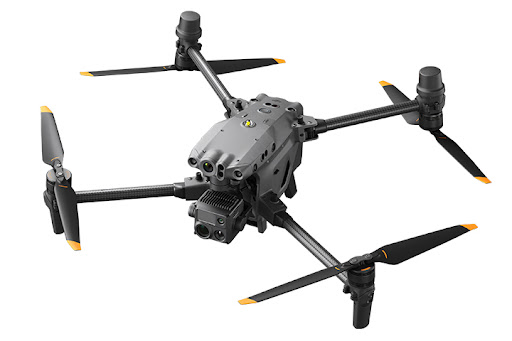
\includegraphics[width=0.5\textwidth]{fig/DJI-M30T.jpg} 
            \caption{โดรน DJI รุ่น M30T}
            \label{fig:DJI-M30T}
        \end{figure} 
    \item \textbf{ESP32 UWB} ทำหน้าที่เป็น Tag ที่ติดตั้งบนโดรน และ Anchor ที่อยู่บนพื้นสำหรับรับ-ส่งสัญญาณ เพื่อคำนวณระยะทาง
        \begin{figure}[htbp] 
            \centering
            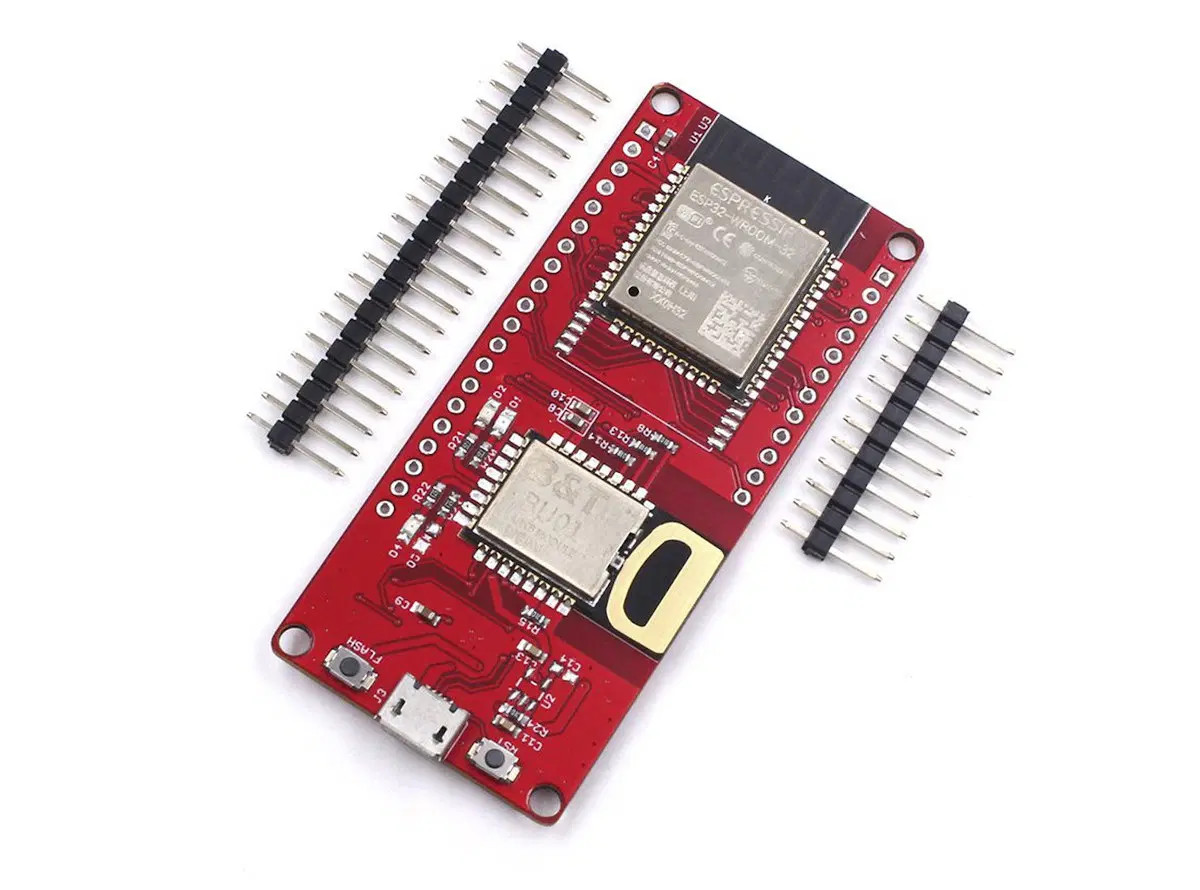
\includegraphics[width=0.3\textwidth]{fig/ESP32-UWB.jpg} 
            \caption{ESP32 UWB}
            \label{fig:ESP32-UWB}
        \end{figure}
    \item \textbf{Laptop Computer} ใช้สำหรับบันทึกข้อมูลการวัด เพื่อนำไปประมวลผลและวิเคราะห์ต่อไป
\end{itemize}

\subsection{\ifenglish Software technology\else เทคโนโลยีด้านซอฟต์แวร์\fi}
\begin{itemize}
    \item \textbf{C++} ใช้พัฒนา Firmware บน ESP32 สำหรับควบคุมโมดูล UWB และคำนวณระยะทาง
    \item \textbf{Python} ใช้สำหรับรับข้อมูลจาก Serial จัดรูปแบบ และบันทึกข้อมูล
    \item \textbf{CSV File} ใช้สำหรับจัดเก็บข้อมูลเพื่อการวิเคราะห์ภายหลัง
\end{itemize}

\section{\ifenglish Project plan\else แผนการดำเนินงาน\fi}

\begin{plan}{11}{2024}{3}{2025}
    \planitem{11}{2024}{11}{2024}{กำหนดหัวข้อและข้อเสนอโครงการ}
    \planitem{12}{2024}{12}{2024}{เลือกอุปกรณ์ที่ใช้ในการทำโครงการ}
    \planitem{12}{2024}{2}{2025}{ศึกษาเครื่องมือและอุปกรณ์ที่ใช้}
    \planitem{2}{2025}{3}{2025}{สรุปผลการสำรวจและเตรียมการพัฒนา}
\end{plan}
\begin{plan}{11}{2025}{3}{2026}
    \planitem{11}{2025}{2}{2026}{พัฒนาโครงสร้างระบบ}
    \planitem{1}{2026}{1}{2026}{ทดสอบระบบในสภาพแวดล้อมจำลอง}
    \planitem{2}{2026}{2}{2026}{ทดสอบระบบในพื้นที่จริง}
    \planitem{3}{2026}{3}{2026}{สรุปผลโครงการและจัดทำรายงาน}
\end{plan}

\section{\ifenglish Roles and responsibilities\else บทบาทและความรับผิดชอบ\fi}
\begin{itemize}
    \item \textbf{นางสาวรวิภา สามห้วย}
        \begin{itemize}
            \item พัฒนาโปรแกรมบน ESP32 เพื่อควบคุมการส่งสัญญาณ UWB
            \item จัดการและวิเคราะห์ข้อมูลที่ได้รับจาก ESP32 UWB (Tag \& Anchor)
        \end{itemize}

    \item \textbf{นางสาววาสิรี นันทจันทร์}
        \begin{itemize}
            \item ออกแบบ 3D PRINT  สำหรับติดตั้ง ESP32 UWB บนโดรน
            \item ประเมินผลการทดสอบที่ได้ในแต่ละครั้ง เพื่อพัฒนาการทดสอบในครั้งถัดไป
        \end{itemize}
\end{itemize}

\section{\ifenglish%
Impacts of this project on society, health, safety, legal, and cultural issues
\else%
ผลกระทบด้านสังคม สุขภาพ ความปลอดภัย กฎหมาย และวัฒนธรรม
\fi}

\subsection{ผลกระทบด้านสังคม}
\begin{itemize}
    \item \textbf{การสนับสนุนงานวิจัยด้านสิ่งแวดล้อม:} ระบบวัดความสูงต้นไม้ที่พัฒนาขึ้นสามารถใช้เป็นเครื่องมือในการเก็บข้อมูลภาคสนาม ซึ่งช่วยเพิ่มประสิทธิภาพในการศึกษาชีวมวลและการดูดซับคาร์บอนของป่าไม้
    \item \textbf{การเพิ่มประสิทธิภาพในการสำรวจพื้นที่:} การใช้โดรนร่วมกับ UWB ช่วยลดข้อจำกัดในการเข้าถึงพื้นที่ป่าที่มีความหนาแน่นสูง ส่งผลให้สามารถเก็บข้อมูลได้รวดเร็วและครอบคลุมมากขึ้น
\end{itemize}

\subsection{ผลกระทบด้านสุขภาพและความปลอดภัย}
\begin{itemize}
    \item \textbf{การลดความเสี่ยงในการปฏิบัติงานภาคสนาม:} การใช้โดรนช่วยลดความจำเป็นในการเข้าถึงพื้นที่เสี่ยง เช่น พื้นที่ลาดชันหรือมีพืชพรรณหนาแน่น ลดโอกาสเกิดอุบัติเหตุจากการสำรวจภาคพื้นดิน
    \item \textbf{ความเสี่ยงจากการใช้งานโดรน:} การบินโดรนในพื้นที่ที่มีสิ่งกีดขวาง เช่น กิ่งไม้ อาจก่อให้เกิดการชนหรือสูญเสียการควบคุม
    \item \textbf{แนวทางลดความเสี่ยง:} ผู้ปฏิบัติงานต้องมีการวางแผนเส้นทางการบิน ตรวจสอบสภาพแวดล้อมก่อนใช้งาน และควบคุมโดรนภายใต้ระยะการมองเห็น (Visual Line of Sight)
\end{itemize}

\subsection{ผลกระทบด้านกฎหมาย}
\begin{itemize}
    \item \textbf{ข้อกำหนดในการใช้โดรน:} การใช้งานโดรนต้องเป็นไปตามกฎหมายและข้อบังคับที่เกี่ยวข้อง เช่น การขึ้นทะเบียนโดรน และการขออนุญาตบินในพื้นที่ที่กำหนด
    \item \textbf{การคุ้มครองข้อมูล:} แม้โครงงานนี้จะเน้นการเก็บข้อมูลความสูงต้นไม้ แต่หากมีการบันทึกภาพหรือพิกัดที่สามารถเชื่อมโยงกับบุคคลหรือทรัพย์สิน ต้องปฏิบัติตามกฎหมายคุ้มครองข้อมูลส่วนบุคคล
\end{itemize}

\subsection{ผลกระทบด้านวัฒนธรรมและสิ่งแวดล้อม}
\begin{itemize}
    \item \textbf{ผลกระทบต่อระบบนิเวศ:} การใช้งานโดรนอาจรบกวนสัตว์ป่าในบางพื้นที่ โดยเฉพาะสัตว์ที่ไวต่อเสียง
    \item \textbf{แนวทางลดผลกระทบ:} ควรหลีกเลี่ยงการบินในช่วงเวลาที่มีสัตว์ป่าทำกิจกรรมสูง และจำกัดระยะเวลาในการบินเพื่อลดผลกระทบต่อระบบนิเวศ
\end{itemize}